

\tikzset{every picture/.style={line width=0.75pt}} %set default line width to 0.75pt        

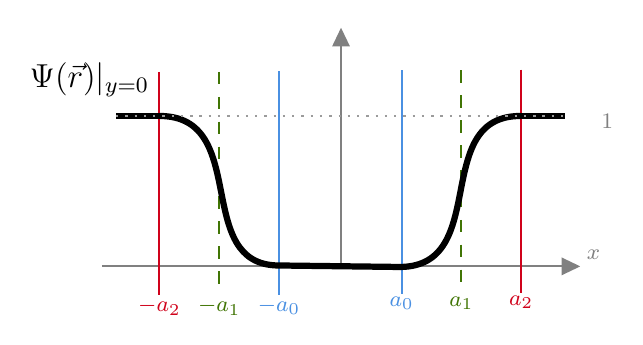
\begin{tikzpicture}[x=0.75pt,y=0.75pt,yscale=-1,xscale=1]
%uncomment if require: \path (0,216); %set diagram left start at 0, and has height of 216

%Straight Lines [id:da6021526004344566] 
\draw [color={rgb, 255:red, 128; green, 128; blue, 128 }  ,draw opacity=1 ]   (191.25,165.61) -- (191.25,53.66) ;
\draw [shift={(191.25,50.66)}, rotate = 90] [fill={rgb, 255:red, 128; green, 128; blue, 128 }  ,fill opacity=1 ][line width=0.08]  [draw opacity=0] (8.93,-4.29) -- (0,0) -- (8.93,4.29) -- cycle    ;
%Straight Lines [id:da09217173902055342] 
\draw [color={rgb, 255:red, 128; green, 128; blue, 128 }  ,draw opacity=1 ]   (76,165.61) -- (303.5,165.61) ;
\draw [shift={(306.5,165.61)}, rotate = 180] [fill={rgb, 255:red, 128; green, 128; blue, 128 }  ,fill opacity=1 ][line width=0.08]  [draw opacity=0] (8.93,-4.29) -- (0,0) -- (8.93,4.29) -- cycle    ;
%Straight Lines [id:da17327433842972684] 
\draw [color={rgb, 255:red, 74; green, 144; blue, 226 }  ,draw opacity=1 ]   (220.42,71.18) -- (220.42,178.87) ;
%Straight Lines [id:da5164207646575634] 
\draw [color={rgb, 255:red, 65; green, 117; blue, 5 }  ,draw opacity=1 ] [dash pattern={on 4.5pt off 4.5pt}]  (249.23,71.18) -- (249.23,178.87) ;
%Straight Lines [id:da9169226167412352] 
\draw [color={rgb, 255:red, 208; green, 2; blue, 27 }  ,draw opacity=1 ]   (278.04,70.82) -- (278.04,178.51) ;
%Straight Lines [id:da08965664307645271] 
\draw [color={rgb, 255:red, 208; green, 2; blue, 27 }  ,draw opacity=1 ]   (103.73,71.91) -- (103.73,179.59) ;
%Straight Lines [id:da855492609907931] 
\draw [color={rgb, 255:red, 65; green, 117; blue, 5 }  ,draw opacity=1 ] [dash pattern={on 4.5pt off 4.5pt}]  (132.54,71.91) -- (132.54,179.59) ;
%Straight Lines [id:da32654209361141806] 
\draw [color={rgb, 255:red, 74; green, 144; blue, 226 }  ,draw opacity=1 ]   (161.36,71.54) -- (161.36,179.23) ;
%Curve Lines [id:da03668323289068964] 
\draw [line width=2.25]    (104.09,93.15) .. controls (148.03,93.51) and (119.22,165.18) .. (161.36,165.18) ;
%Curve Lines [id:da11356455536917842] 
\draw [line width=2.25]    (277.68,93.15) .. controls (234.11,93.15) and (263.64,165.54) .. (219.7,165.9) ;
%Straight Lines [id:da3940509531593688] 
\draw [line width=2.25]    (161.36,165.18) -- (219.7,165.9) ;
%Straight Lines [id:da4374758728023367] 
\draw [line width=2.25]    (277.68,93.15) -- (298.93,93.15) ;
%Straight Lines [id:da7083449686833048] 
\draw [line width=2.25]    (82.84,93.15) -- (104.09,93.15) ;
%Straight Lines [id:da2928034275546325] 
\draw [color={rgb, 255:red, 155; green, 155; blue, 155 }  ,draw opacity=1 ][line width=0.75]  [dash pattern={on 0.84pt off 2.51pt}]  (82.84,93.15) -- (298,93.15) ;

% Text Node
\draw (308.24,156.39) node [anchor=north west][inner sep=0.75pt]  [font=\footnotesize,color={rgb, 255:red, 128; green, 128; blue, 128 }  ,opacity=1 ]  {$x$};
% Text Node
\draw (100.22,85.51) node [anchor=south east] [inner sep=0.75pt]  [font=\large,color={rgb, 255:red, 0; green, 0; blue, 0 }  ,opacity=1 ]  {$\Psi(\vec{r}) |_{y=0}$};
% Text Node
\draw (220.42,178.91) node [anchor=north] [inner sep=0.75pt]  [font=\footnotesize,color={rgb, 255:red, 74; green, 144; blue, 226 }  ,opacity=1 ]  {$a_{0}$};
% Text Node
\draw (249.23,178.91) node [anchor=north] [inner sep=0.75pt]  [font=\footnotesize,color={rgb, 255:red, 65; green, 117; blue, 5 }  ,opacity=1 ]  {$a_{1}$};
% Text Node
\draw (278.04,178.55) node [anchor=north] [inner sep=0.75pt]  [font=\footnotesize,color={rgb, 255:red, 208; green, 2; blue, 27 }  ,opacity=1 ]  {$a_{2}$};
% Text Node
\draw (161.36,179.27) node [anchor=north] [inner sep=0.75pt]  [font=\footnotesize,color={rgb, 255:red, 74; green, 144; blue, 226 }  ,opacity=1 ]  {$-a_{0}$};
% Text Node
\draw (132.54,179.63) node [anchor=north] [inner sep=0.75pt]  [font=\footnotesize,color={rgb, 255:red, 65; green, 117; blue, 5 }  ,opacity=1 ]  {$-a_{1}$};
% Text Node
\draw (103.73,179.63) node [anchor=north] [inner sep=0.75pt]  [font=\footnotesize,color={rgb, 255:red, 208; green, 2; blue, 27 }  ,opacity=1 ]  {$-a_{2}$};
% Text Node
\draw (319.5,100.76) node [anchor=south] [inner sep=0.75pt]  [font=\footnotesize,color={rgb, 255:red, 128; green, 128; blue, 128 }  ,opacity=1 ]  {$1$};


\end{tikzpicture}
